\documentclass[a4paper]{article}

\usepackage[margin=2cm]{geometry}
\usepackage{fontspec}
\usepackage[english]{babel}

\usepackage{amsmath, amsfonts}

\usepackage{tikz}
\usetikzlibrary{positioning}
\tikzset{main node/.style={circle,fill=blue!20,draw,minimum size=1cm,inner sep=0pt},
}

\setlength{\parindent}{0pt}

\title{Entrega puntuable d'Ampliació d'Algorísmia \\ \texttt{Maximum planar subgraph}}
\author{Marc Asenjo i Ponce de León \and Arnau Canyadell i Miquel \and Joan Marcè i Igual}
\date{}

\begin{document}

\maketitle

\section{Descripció del problema}
El problema del \texttt{Maximum planar subgraph} es defineix de la manera següent:

Donat un graf $G=(V,E)$, computar un subgraf planar $G'=(V,E')$ amb el màxim nombre d'arestes.

\subsection{Exemple}
Un exemple d'instància del problema és el problema donat pel graf $G$, on $G$ és la clique de $|V|=4$.

Donat que $G$ no és un subgraf planar, s'ha d'eliminar com a mínim alguna aresta, com es mostra en la figura següent.

\begin{figure}[!h]
	\centering
	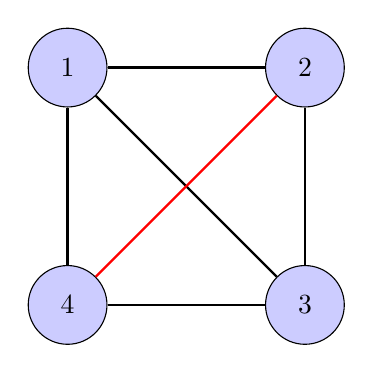
\begin{tikzpicture}
	\node[main node] (1) {$1$};
	\node[main node] (2) [right = 2cm  of 1] {$2$};
	\node[main node] (4) [below = 2cm  of 1] {$4$};
	\node[main node] (3) [right = 2cm  of 4] {$3$};
	
	\path[draw,thick]
	(1) edge node {} (2)
	(2) edge node {} (3)
	(3) edge node {} (4)
	(4) edge node {} (1)
	(1) edge node {} (3)
	(2) edge[red] node {} (4)
	;
	\end{tikzpicture}	
\end{figure}

\section{Problemes derivats}
\subsection{Problema decisional: \texttt{Is maximum planar subgraph}}
Donat un graf $G=(V,E)$ i un subgraf planar de $G$, $G'=(V,E')$, dir si $G'$ és un \texttt{Maximum planar subgraph} de $G$.

\subsection{Problema parametritzat: \texttt{K-planar subgraph}}
Donat un graf $G=(V,E)$ i un enter $k$, computar un subgraf planar $G'=(V,E')$ amb $|E'|=k$.

\end{document}